% Usar el tipo de documento: Artículo científico.
\documentclass[11pt,a4paper,hidelinks]{article}

% Cargar mensajes en español.
\usepackage[spanish,es-noquoting]{babel}

% Usar codificación utf-8 para acentos y otros.
\usepackage[utf8]{inputenc}
\usepackage[T1]{fontenc}
\usepackage{lmodern}

% Dimensiones de los márgenes.
\usepackage[margin=1.8cm]{geometry}

% Insertar porciones de código
\usepackage{listings}

% Comenzar párrafos con separación no indentación.
\usepackage{parskip}
%enlaces
\usepackage{hyperref}
% Usar gráficos
\usepackage{graphicx}
\usepackage{caption}
\usepackage{subcaption}
%
% Usar contenedores flotantes para figuras.
\usepackage{float}

% Carpeta de las imágenes.
\graphicspath{{img/}}

% Matemáticas
\usepackage{amsmath}
\usepackage{mathtools}

% Símbolos del sistema internacional
\usepackage{siunitx}

% Gráficas con pgf
\usepackage{pgfplots}

% Tablas con varias filas unidas
\usepackage{multirow}

% Tablas en el texto
\usepackage{wrapfig}

\begin{document}
%\maketitle
\begin{center}
\begin{huge}
\textbf{Trak}
\end{huge}
\\[10pt]
\textbf{Rodrigo Arias Mallo}\\
rodrigo.arias@udc.es
\end{center}

\part{Diseño artístico}
\section{Descripción}
Trak es un videojuego 3D de conducción extrema. Se caracteriza por las altas 
velocidades y los saltos en el aire. Está ambientado en la serie de videojuegos 
TrackMania. Los aspectos de conducción así como el modelo de pistas siguen el 
mismo estilo.

\section{Mapas}
Incluye una serie de mapas que se pueden jugar, y en los que se registrarán los 
mejores tiempos. Adicionalmente, nuevos mapas pueden ser creados o compartidos.

Los mapas están contituídos de bloques de diferentes tipos de tramos. Existen 
tramos rectos, curvos o con saltos. Además de los bloques especiales de inicio y 
fin de carrera.

\section{Mecánica de juego}
El juego es sencillo. Tan sólo elige un nombre de jugador, un mapa y trata de 
conseguir el mejor tiempo posible. Para ello has de emplear una buena técnica de 
conducción, acelerando lo máximo posible y teniendo especial cuidado en no 
chocar con las paredes o volcar.

\begin{center}
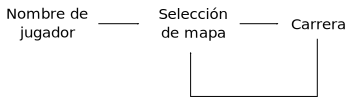
\includegraphics{fases}
\end{center}

Incluye un selector de mapas, que explora todos aquellos que se encuentren 
disponibles, lo que permite añadir nuevos mapas fácilmente, y seleccionarlos 
desde el juego.

\newpage
\part{Diseño interno}
\section{Introducción}
Trak está íntegramente desarrollado en Blender, un editor de modelos 3D, que 
incluye un motor gráfico basado en el motor de físicas Bullet.

A continuación se detallará el diseño de todos los componentes que confoman el 
juego, tanto el vehículo como los mapas y menús.

\section{Vehículo}
\subsection{Estructura}
El vehículo está formado de una parte estética, que se mostrará en el juego, y 
una representación más simple, empleada en las físicas. Todos los componentes 
del vehículo forman un grupo, que se puede instanciar en un mapa, permitiendo la 
abstracción de los detalles del mismo.

En la parte estética se encuentra la carrocería, y las cuatro ruedas que tienen 
desactivada la colisión con otros objetos. Además han sido simplificados 
estructuralmente, para acelerar el renderizado. De esta forma los 215.000 
vértices se reducen a un 16\%: 35.000.

El aspecto del vehículo tras la reducción de vértices:

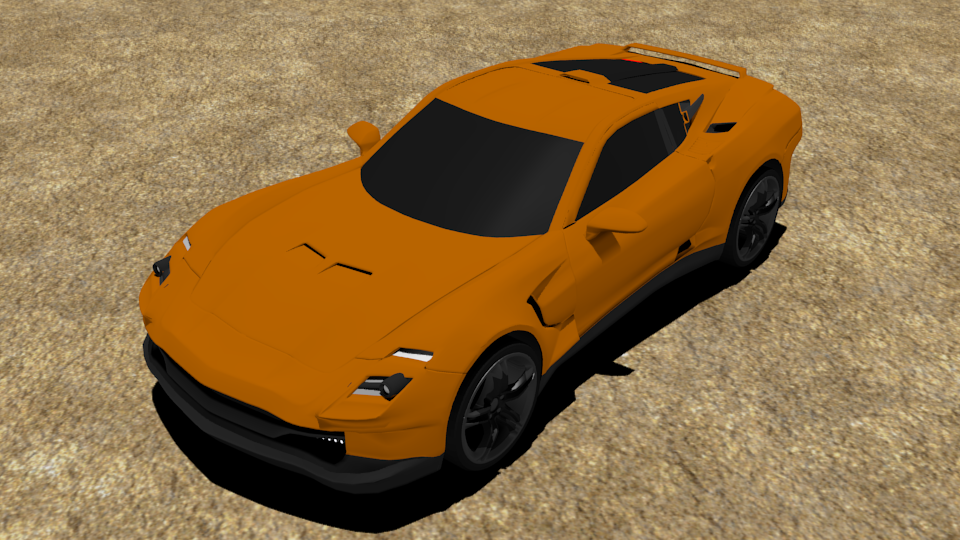
\includegraphics[width=\textwidth]{coche}

La estructura que se muestra a continuación proporciona la simplificación 
adecuada para realizar colisiones con el vehículo sin la complejidad de la 
carrocería.

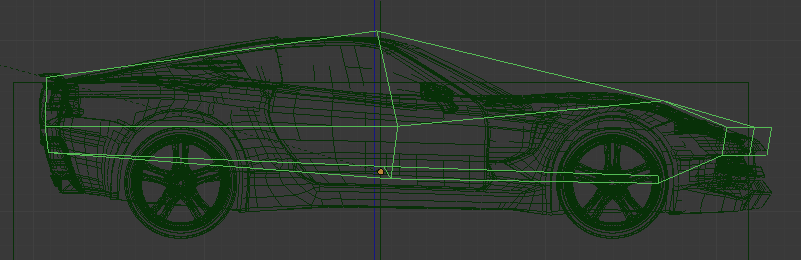
\includegraphics[width=\textwidth]{vehiculo-colision}

El punto amarillo en la parte inferior de la carrocería es el centro de masa. Se 
encuentra cerca del suelo para mejorar la estabilidad al tomar las curvas.


\subsection{Control}
El control del vehículo se realiza mediante un controlador de vehículos que 
incluye Bullet. De esta forma se simplifica la hercúlea tarea de simular el 
comportamiento de un coche, a una tarea compleja; la de ajustar el 
comportamiento al de un coche real.

Existen diferentes parámetros que configuran el control del vehículo.
En la tabla, se esquematizan los parámetros para una visión más clara.
\begin{center}
\begin{tabular}{ | c | l | }
	\hline
	\multirow{2}{*}{Fuerza}
	& Motor \\
	& Frenos \\
	\hline
	\multirow{4}{*}{Suspensión}
	& Rigidez \\
	& Longitud \\
	& Expansión \\
	& Compresión \\
	\hline
	\multirow{3}{*}{Ruedas}
	& Radio \\
	& Fricción \\
	& Influencia \\
	\hline
	\multirow{5}{*}{Vehículo}
	& Dimensiones \\
	& Centro de masa \\
	& Masa \\
	& Gravedad \\
	& Escala \\
	\hline
\end{tabular}
\end{center}
\begin{description}
	\item[Fuerza de motor] Simula el efecto del motor. Valores altos 
	provocarán una aceleración mayor.
	\item[Fuerza de frenada] Simula el rozamiento de los frenos contra las 
	ruedas. Valores más altos implicarán una deceleración mayor.
	\item[Rigidez] Resistencia a la deformación de la suspensión. Es la 
	constante del muelle, y relaciona la distancia de compresión con la 
	fuerza aplicada.
	\item[Longitud] Es la longitud de la suspensión. Valores más altos 
	permitirán un recorrido mayor.
	\item[Expansión] Controla el suavizado de la expansión de la suspensión.  
	Valores altos expandirán la suspensión de forma más lenta.
	Debe estar comprendido entre 0 y 1 para $K$ en 
	$2K\sqrt{\texttt{rigidez}}$
	\item[Compresión] Configura el suavizado de compresión de la suspensión.  
	Mismo intervalo, $K = 0.0$ sin suavizar, $K = 1.0$ suavizado crítico. Se 
	recomienda K entre 0.1 y 0.3. Debe ser menor que la expansión.
	
	\item[Radio de rueda] Cuanto mayor sea el radio mayor la velocidad pero 
	menor el par.
	\item[Fricción de la rueda] Determina el agarre de la rueda. Un valor 
	más alto impedirá que la rueda se desplace horizontalmente en las 
	curvas. Puede provocar que el vehículo vuelque.
	\item[Influencia de la rueda] Permite disminuir el par transmitido a la 
	rueda antes de que provoque que el coche vuelque. Valores altos 
	disminuyen el efecto, haciendo más inestable la conducción.
	\item[Dimensiones] La anchura del vehículo determinará su estabilidad.  
	La longitud, su habilidad para sobrepasar obstáculos, así como el radio 
	de giro. Y la altura, determinará la estabilidad al chocar lateralmente.
	\item[Centro de masa] Es un punto que se comporta como toda la 
	carrocería, en cuanto a las fuerzas aplicadas a ella se refiere. Su 
	altura determinará la estabilidad. Valores más altos, menor estabilidad.
	\item[Masa] Permite aumentar la inercia ante choques y reducir la 
	aceleración.
	\item[Gravedad] Determina la aceleración del vehículo hacia el suelo.  
	Valores muy altos pueden provocar una simulación errática.
	\item[Factor de escala] Es la diferencia de tamaño entre el coche del 
	mundo real y el del juego. Es muy importante para calibrar el 
	comportamiento en un mundo más pequeno, y aumentar así la sensación de 
	velocidad.  Además las físicas no funcionan adecuadamente para objetos 
	muy pequeños.
\end{description}

\subsection{Lógica}
El vehículo controla la cámara, el teclado, y contiene la programación para 
comenzar y terminar una carrera. Esta decisión de diseño se debe a que estará 
presente en todos los mapas, y por lo tanto, será un elemento reutilizable, y 
aplicable a nuevos mapas.

Primero el vehículo busca en la escena dos bloques especiales, que contienen las 
propiedades de comienzo y fin de carrera. Luego se sitúa en la posición de 
comienzo, y arranca el tiempo junto con la carrera. Para llegar a la meta, 
comprueba la colisión con el bloque de fin de carrera.

A través del teclado se calcula la fuerza que ha de aplicarse al motor, y la 
dirección, así como el giro de la dirección. Este giro se calcula mediante un 
función que relaciona la velocidad con el giro máximo de la dirección. De esta 
forma, al viajar a altas velocidades se realiza un giro suave, frente a un giro 
cerrado a baja velocidad. De modo que para tomar una curva cerrada es necesario 
reducir la velocidad.

\section{Mapas}
El juego ha sido creado con la intención de que los mapas se puedan construir de 
una forma sencilla. Para ello, existe una colección de bloques que constituyen 
tramos de la trazada con diferentes formas.

En la figura se muestran los bloques en verde, y el circuito en naranja. Todo el 
circuito ha sido creado a partir de la sucesiva concatenación de bloques.

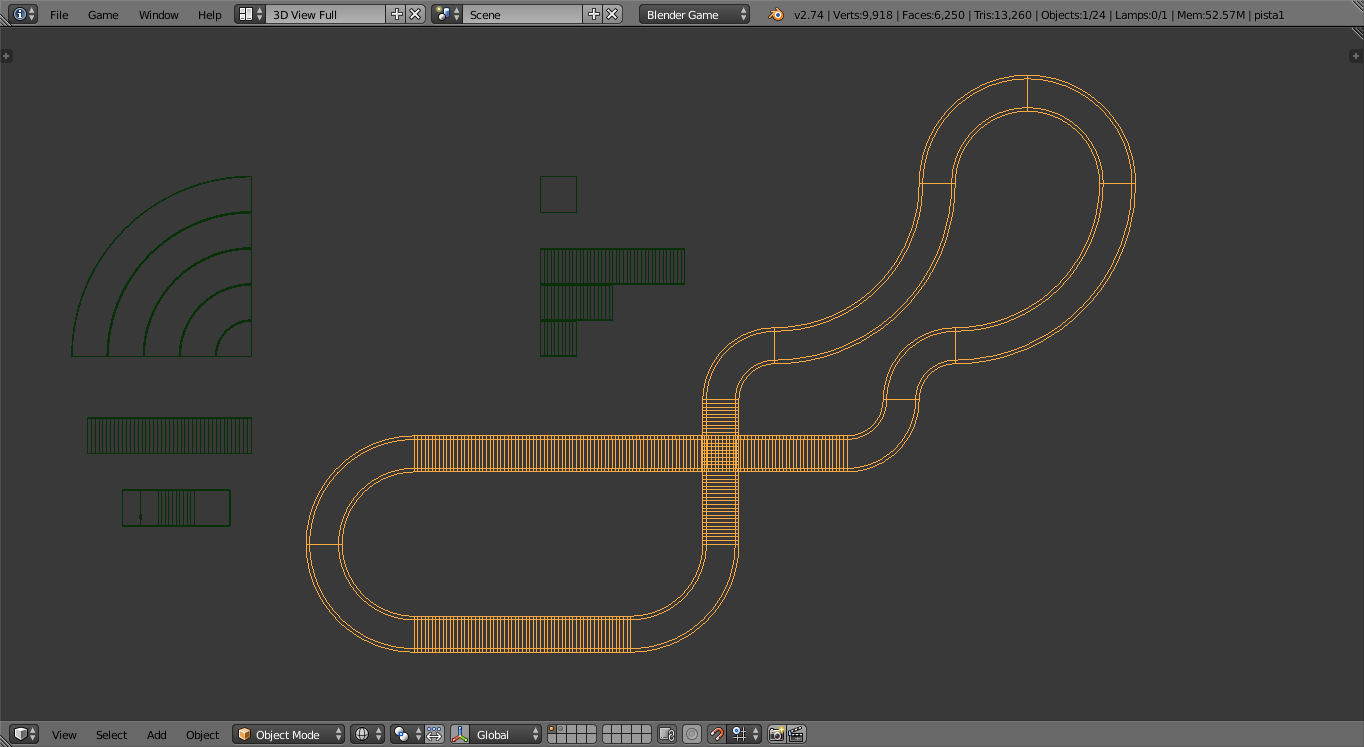
\includegraphics[width=\textwidth]{bloques}

De esta forma, se logra elaborar un método sencillo y rápido para crear nuevas 
pistas.

Además, cada bloque de trazada está formado de la modificación de un forma base.  
La forma base, define el perfil de la trazada, los materiales y las texturas que 
se asignarán a cada parte de la carretera. De modo que para construir cualquier 
pieza, basta con indicar el giro o la extrusión a la forma base, y obtener el 
bloque deseado. La forma base se muestra en la siguiente figura.

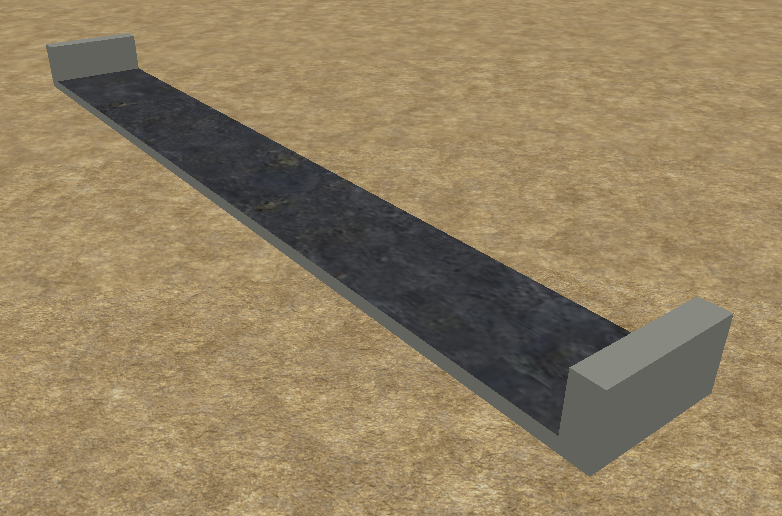
\includegraphics[width=\textwidth]{base}

Esto permite la rápida edición de bloques en grupo. Al cambiar la textura del 
suelo en la forma base, todos los bloques que hayan sido creados a partir de 
esta forma, se modificarán automáticamente. También es posible cambiar la forma 
o el tamaño.

Es un claro ejemplo de herencia en el paradigma de orientación a objetos, 
centrado en la reutilización de código, en este caso de modelos.

Algunas piezas contruídas de esta forma se muestran en esta imagen:

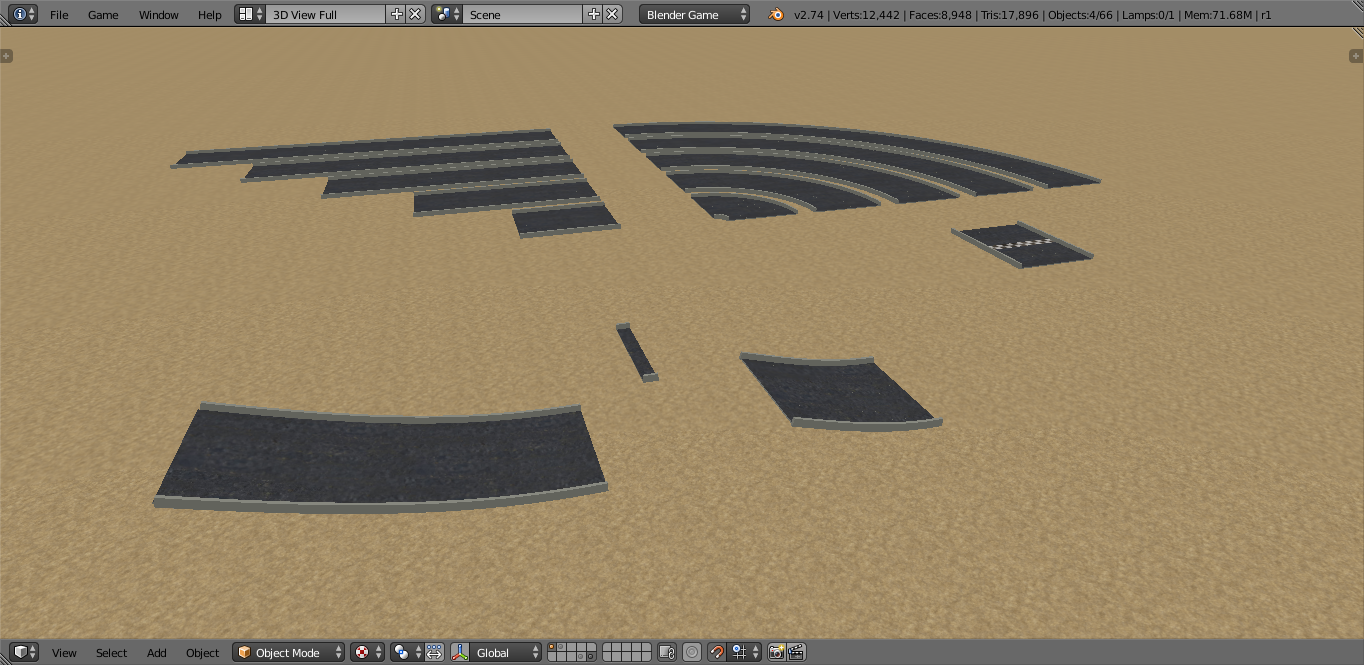
\includegraphics[width=\textwidth]{piezas}

Adicionalmente, cada pieza permite ser instanciada en un mapa, de modo que el 
diseño de una carrera se abstrae de las partes internas de cada bloque, 
mostrándose como un componente único.

\subsection{Bloques especiales}
Algunos bloques tienen propiedades especiales, que son reconocidas por el 
vehículo.

El bloque de comienzo, indica la posición desde donde ha de comenzar la partida, 
así como el punto para restablecer la carrera. Contiene la propiedad 
\texttt{start}, y sitúa el centro del objeto en el punto en el que ha de 
aparecer el vehículo.

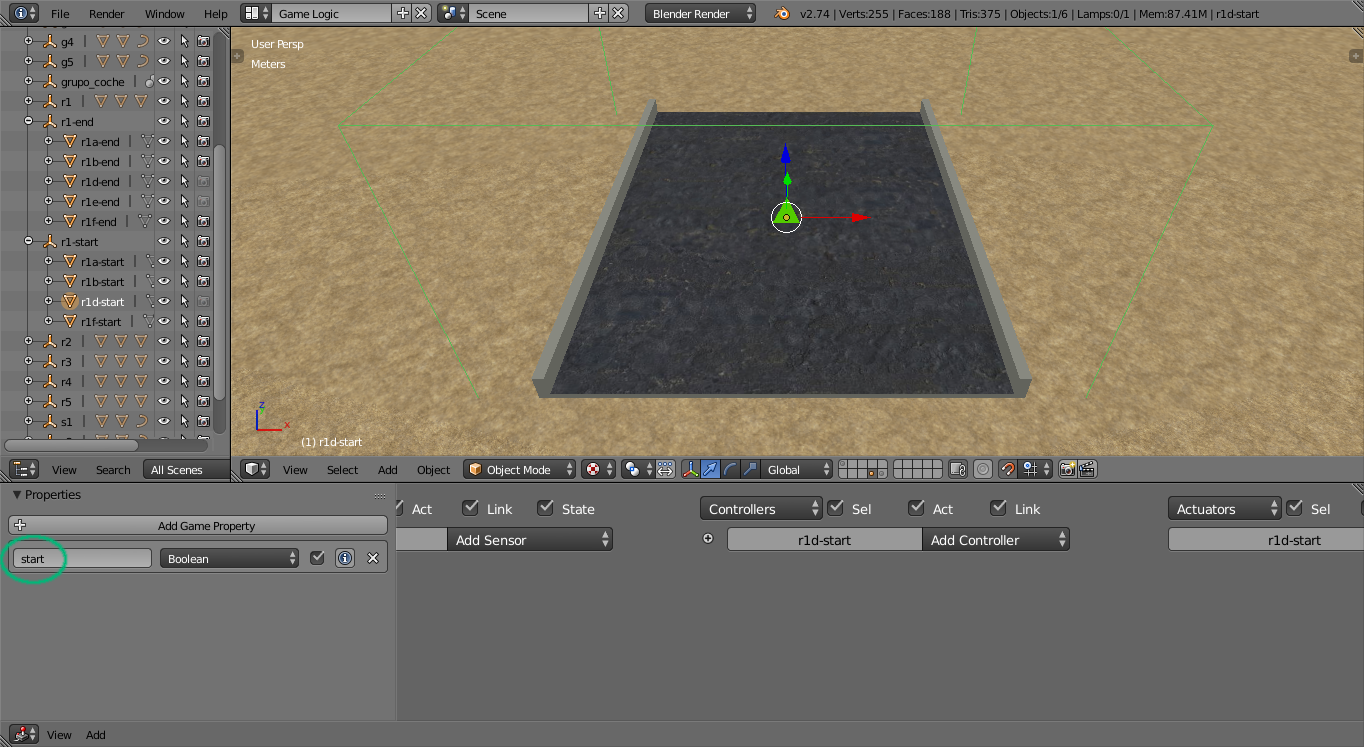
\includegraphics[width=\textwidth]{start}

El bloque de meta, contiene un objeto rectangular que actúa como colisionador.  
Cuando el vehículo lo atraviesa, indica que ha llegado a la meta. La altura del 
objeto permite entrar en la meta, sin necesidad de tocar el suelo, dado que en 
algunos mapas el coche pasará por el aire. Se muestra a continuación en verde.

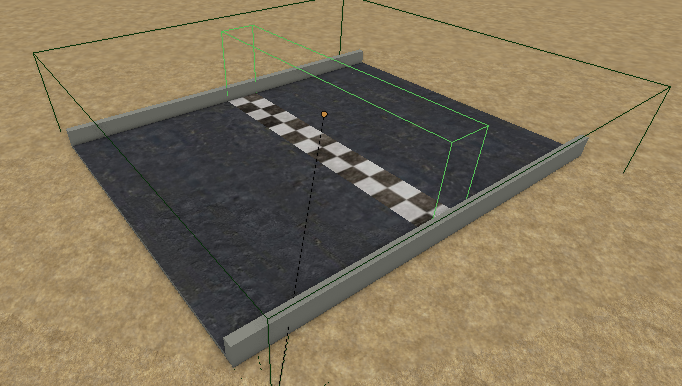
\includegraphics[width=\textwidth]{end}

\section{Estructura del proyecto}
La ubicación de cada componente del videojuego, se ha clasificado para mantener 
el juego ordenado. Se ha seguido una jerarquía de directorios.

\begin{center}
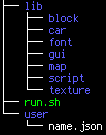
\includegraphics[scale=0.8]{dir}
\end{center}

Cada mapa se guarda en un fichero propio, así como en un directorio propio. En 
el directorio de cada mapa se encuentran las puntuaciones más altas de dicha 
pista. Esto permite compartir un mapa, junto con las puntuaciones guardadas.  
Todos los mapas están en \texttt{lib/map}.

Los bloques están ubicados aparte de los mapas en \texttt{lib/block}, 
permitiendo la edición de todos los bloques en los mapas de forma automática.

El vehículo se escuentra en un directorio diferente \texttt{lib/car}, con la 
idea de permitir añadir nuevos vehículos en el futuro.

Todos los scripts del juego están colocados en un directorio común 
\texttt{lib/script}, para permitir que sean reutilizados en diferentes mapas o 
vehículos.

En \texttt{user/} se encuentra la información relativa al usuario, que variará 
en cada juego. Se ha situado aparte para permitir añadir más configuraciones en 
el futuro. Almacena el nombre de usuario en \texttt{user/name.json}.

Las pantallas de menús (GUI) están ubicadas en \texttt{lib/gui}, donde cada 
pantalla se almacena en un directorio independiente.

\section{GUI}
El juego dispone de varias pantallas de menús que permiten editar propiedades y 
seleccionar los circuitos, así como mostrar las mejores puntuaciones. Gracias al 
módulo bgui, la compleja tarea de colocar cada elemento en su sitio, se vuelve 
más sencilla, ya que cuenta con widgets como botones, entradas de texto o 
marcos.

\subsection{Jugador}
Este menú muestra una entrada de texto que permite elegir el nombre del jugador.  
Una vez elegido, al presionar Enter se confirma la selección, y se muestra la 
siguiente escena, la selección del mapa.

El jugador seleccionado será el que aparecerá en las puntuaciones a medida que 
se completen las carreras. Además, al reiniciar el juego, el jugador 
seleccionado se sigue manteniendo permitiendo continuar con sólo pulsar Enter, o 
cambiar de jugador.
\begin{center}
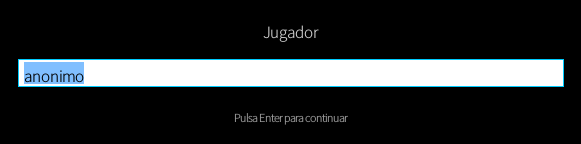
\includegraphics[scale=0.5]{jugador}
\end{center}

\subsection{Selección de mapa}
Permite elegir un mapa, y explorar los que están disponibles. También muestra 
las mejores puntuaciones de cada mapa.

La navegación ha sido diseñada en páginas, que visualiza 5 mapas cada vez.

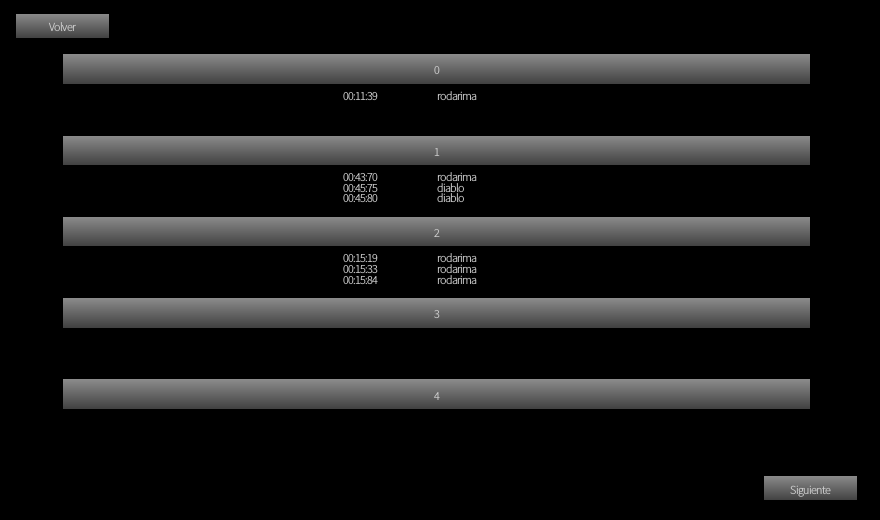
\includegraphics[width=\textwidth]{browse}


\section{HUD}
En la pantalla de conducción se superpone un HUD (Heads-Up Display), que muestra 
el tiempo de carrera y una notificación al llegar a la meta. Se encuentra en una 
escena superpuesta a la visión de la cámara de conducción.

\begin{center}
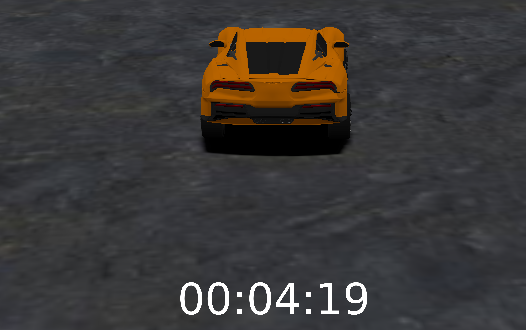
\includegraphics[scale=0.5]{hud}
\end{center}

Al llegar a la meta, el tiempo se detiene y se muestra la notificación de 
llegada. Sin embargo el juego continúa durante unos segundos, permitiendo que el 
vehículo pueda continuar su camino, y chocar si procede. Este detalle es 
característico de Trackmanía.

\section{Controles del juego}
En los menús, la selección de los botones se realiza mediante el ratón. En 
cualquier parte del juego, pulsar Q para salir. Pulsar Escape para volver al
menú anterior o para abandonar la carrera.

El vehículo se controla mediante las flechas del teclado. Derecha e izquierda 
para la dirección. Adelante y atrás para la acelerar marcha adelante o atrás.  
Para usar el freno de mano emplear Control.

Backspace restaura el vehículo en el comienzo de la carrera y reinicia el mapa.

\section{Instalación y ejecución}
Para ejecutar el juego es necesario instalar Blender. Una vez instalado, 
dirigirse a la carpeta del proyecto y ejecutar:

\texttt{\$ ./run.sh}.

Adicionalmente, los mapas se pueden abrir directamente con Blender, y presionar 
P para jugar dentro del editor.

\section{Agradecimientos}
El desarrollo de este videojuego no habría sido posible sin la ayuda de:
Kester Maddock por su aporte acerca de los diferentes parámetros de un vehículo, 
en Bullet. A Mitchell Stokes (Moguri), por la creación de la interfaz de menus 
que incluye el juego. A todo el equipo detrás de la biblioteca de físicas Bullet 
que es el corazón de toda la simulación de conducción. Al de Blender, y sobre 
todo al enorme trabajo de documentación para ofrecer un contenido más claro. A 
Monster y Bananaft de blenderartists, que gracias a sus ejemplos y tutoriales ha 
sido posible la construcción de todo el juego.

\end{document}
